% \documentclass[letterpaper,12pt]{article}
\documentclass[a4paper,10pt]{article}
\usepackage[total={18cm,20cm}, top=1.5cm, left=1.5cm]{geometry}
\usepackage[spanish]{babel}
\usepackage[utf8]{inputenc}
% \usepackage[latin1]{inputenc}
\usepackage[T1]{fontenc}
\usepackage{graphicx}
\usepackage{subfigure}
\usepackage{fancyhdr}
\usepackage{setspace}
\usepackage{hyperref}
\usepackage{multirow}
\usepackage{float}

\renewcommand{\baselinestretch}{1.5}
\pagestyle{fancy}
\rhead{
\includegraphics[width = .055\textwidth]{imagenes/LogoBase.png}}
\lhead{\textit{Social Data Mining \& statistics}}

% \fancyfoot[R]{\includegraphics[width=5mm]{./imagenes/logo.png}}

\title{Comparación de los efectos de la disminución de posteos sobre las estadísticas del público e interacciones de 
una cuenta de Facebook pública}
\author{Social Data Mining \& Statistics \\
        Base10\\
        \scriptsize Dorantes Nieto Fernando ferdorantes@base10.mx}
% \subtitle{LatReach}
\date{}


\begin{document}
\maketitle

\begin{abstract}

Actualmente la mitad de la población mundial utiliza internet, de
todas las páginas existentes, Facebook es de las que tienen un mayor número
de usuarios. Facebook ayuda a conectar a los seres humanos y por 
ser una red social muy utilizada, puede servir como canal para
realizar estrategias de mercadeo.
De manera general muchas empresas postean un determinado número de 
campañas en Facebook, el número de posteos va de la mano con el número
de seguidores de una página en particular.
Para el caso particular de SEAT de México, se postea 4 veces al día.
No obstante con el fin de mejorar la calidad de los posteos, se pretende saber 
los efectos de postear 3 veces en vez de 4.
Se realizó un experimento de 4 semanas, donde las primeras dos se
posteó 3 veces y en las siguientes dos 4 veces. 
Se midió la interacción, el alcance, el enganche y las impresiones, posteriormente se realizaron 
modelos lineales generalizados y análisis de varianza para la comparación entre semanas.
Para la mayoría de las interacciones, se encontraron diferencias significativas,
dando como resultado que publicar cuatro veces genera mayor interacción que publicar 3 veces.
Sin embargo, para el caso de las demás métricas (alcance, enganche e impresiones) no 
existen diferencias significativas, esto indica que postear tres o cuatro posteos
no modifica en gran medida el número de usuarios alcanzados o enganchados.
El disminuir, aumentar o mantener el número de posteos, va de la mano con las necesidades de los mercadólogos de
SEAT donde para mantener el enganche y alcance, postear tres veces parece ser suficiente, 
sin embargo para la interacción no parece recomendable postear solo tres veces, no obstante esto 
podría mejorarse si se toman en cuenta otras variables para mejorar la calidad de los posteos de SEAT.\\
\textbf{Palabras clave:}  Facebook, posteos, alcance, enganche, interacción, impresiones, mercadeo.

\end{abstract} 
  \\[-2cm]
\section{Introducción}
Hasta el mes de Junio de 2016, la población humana era de 7,340,156,492 personas, 
de toda esa población el 50.1 \% (3,675,824,813) utilizaban internet
(Internet World Stats, 2016).\\
De la gran cantidad de páginas que existen en Internet, Facebook es una de las 
más utilizadas, con un promedio de 1040 millones de personas conectadas diariamente 
a este sitio web (Facebook statistics, 2016).\\
Facebook es una red social, al igual que otros sitios web como Twitter o Instagram,
no obstante, Facebook lidera en el número de usuarios (Smarthinsights, 2016).
La popularidad y por ende el uso de las redes sociales obedece a que los 
seres humanos son altamente dependientes del soporte social de otros seres
de su misma especie. Por lo tanto, las redes sociales satisfacen dos necesidades
primordiales de los seres humanos: Necesidad de autorepresentación y la necesidad
de pertenencia a un grupo (Nadkarni y Hofmann, 2012).\\
Más allá del impacto social y de comportamiento que pueda tener Facebook,
esta red social puede ser utilizada para diversos fines, que van desde la investigación 
y finalizando con el mercadeo (marketing) (Wilson et al, 2012).
Para el caso del mercadeo, Facebook es uno de los sitios en los cuales
las personas pasan una gran cantidad de su tiempo, por lo tanto podría considerarse
un gran canal para dar anuncios de diversas empresas (Roshnee y Fowdar, 2013).
En otros aspectos, Facebook puede ayudar a comprender el 
comportamiento de los potenciales consumidores de varias empresas.
Por otro lado es posible realizar estrategias específicas para los potenciales
consumidores o seguidores de las redes sociales de alguna marca en particular (Casteleyn et al, 2009).\\
Sin embargo, la forma de interacción entre empresa y consumidor, cambia
con el tiempo, debido a diversos factores, uno de ellos es el cambio constante
del algoritmo de Facebook encargado de regular la sección de noticias de cada usuario (\textit{EdgeRank}).
De esta manera, las empresas deben cambiar regularmente la manera en como interactúan
con sus seguidores.
\\ [0.5cm]
La forma más común de interactuar con los seguidores de cierta empresa es realizar
posteos(publicar imágenes, texto, video) en los perfiles públicos de las mismas empresas.
Estos posteos son la base para poder obtener las diversas métricas que las empresas
necesitan para poder comprender el comportamiento  de sus usuarios o potenciales
compradores.\\
Postear demasiado o poco, puede resultar arriesgado, puesto que en promedio 
cada usuario de Facebook tiene 1500 publicaciones nuevas
diarias en su muro, ya sea de sus amigos, seguidores o sitios que el usuario sigue (Facebook business, 2013).
En general, del gran número de publicaciones que un usuario tiene en su muro, solo puede ver un pequeño porcentaje de estas.

De manera general, el número de posteos realizados por determinada empresa va de la mano
con el número de usuarios que siguen a la misma. Patel (2012) propuso que si se tiene al menos
10,000 seguidores lo ideal sería postear al menos dos veces al día y eso te garantizaba una 
buena suma de ``clicks''  e interacciones.

No obstante con el cambio constante del algoritmo \textit{EdgeRank}, actualmente es
muy dificil garantizar una gran interacción.
Muchos sitios recomiendan que para tener una gran interacción, se necesitan de al menos
dos características importantes para cada posteo: Un gran incentivo (foto, video, gif) 
y una corta descripción que incite a realizar una acción (``click'' p.ej).\\
Para nuestro caso en particular, SEAT  de México se esfuerza en realizar cuatro posteos
diarios. Contando con 1 millon 600 mil seguidores a la fecha.
Para mejorar la calidad de los posteos y obtener la misma o una mayor cantidad de métricas
positivas en la cuenta de Facebook de SEAT.
Se propone un experimento que consiste en disminuir el número de posteos a tres por día para
comprender la dinámica de las interacciones y estadísticas del público  para la cuenta de SEAT.
Para realizar dicho experimento, se planea comparar las interacciones y estadísticas del público 
producidas en dos semanas con tres posteos diarios con las interacciones y estadísticas del público de dos semanas con cuatro posteos.



\section{Objetivo general}
Determinar los efectos en las interacciones y las estadísticas del público al realizar tres y cuatro posteos diarios en la 
cuenta de Facebook de SEAT de México.


\section{Objetivos particulares}
  \begin{itemize}
   \item[$*$] Conocer el enganche (``engagement'') y alcance producto de la disminución de las publicaciones.
   \item[$*$] Conocer la cantidad de comentarios, reacciones, número de veces que se comparte una publicación al disminuir las publicaciones.
   \item[$*$] Comparar el número interacciones de dos semanas con tres posteos al día contra otras dos de  cuatro posteos diarios.
  \end{itemize}


\section{Metodología}
El experimento se realizó en cuatro semanas, el periodo de tiempo comprende del 6 de Marzo al 4 de Abril de 2017 (28 días).

En las  primeras dos  semanas del experimento se realizaron tres posteos al día,
las siguientes dos semanas se posteó 4 veces al día (Figura 1).
Para cada posteo, se tuvo un tiempo de espera de 24 horas desde que se liberó cada posteo en Facebook, 
una vez que pasó este periodo de tiempo, se midieron el número de interacciones,
el alcance, el enganche  y las impresiones del posteo, además de las impresiones hacia los fans
del posteo. 
También por cada día se calculó el enganche general.

Se esperaba un total de 98 datos por cada variable (42 en la primera semana y 56 para la segunda),
sin embargo en la segunda semana del experimento solo se pudo postear dos veces en un día por lo que 
el tamaño de la muestra para las semanas de 3 posteos es de 41. Esta falta de datos se ha contemplado para
los análisis estadísticos.

\begin{figure}[H]
  \begin{center}
   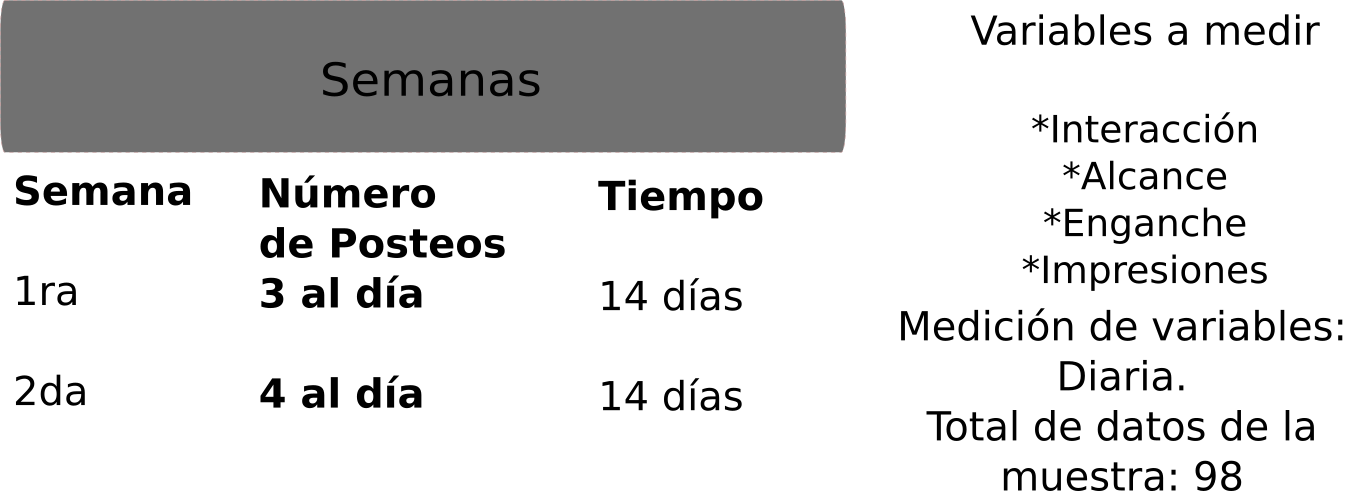
\includegraphics[width=.75\textwidth]{imagenes/dibujoExperimentoRenovado.png}
   \caption{Diseño experimental.}
  \end{center} 
\end{figure}

Las variables tomadas en cuenta fueron las siguientes:
\begin{itemize}
 \item[$*$] Interacciones
  \subitem Interacción total (Suma de todas las reacciones, comentarios y número de veces compartido)
  \subitem Reacciones totales (Suma de todas las reacciones)
  \subitem Reacciones sin ``Me gusta''
  \subitem Comentarios
  \subitem Número de veces compartido (``Shares'' en inglés)
  \subitem ``Me gusta''
  \subitem ``Me encanta''
  \subitem ``Me divierte''
  \subitem ``Me sorprende''
  \subitem ``Me entristece''
  \subitem ``Me enoja''
 \item[$*$] Enganche por posteo
 \item[$*$] Alcance por posteo
 \item[$*$] Impresiones por posteo (totales y únicas)
 \item[$*$] Impresiones hacia los fans (totales y únicas)
 \item[$*$] Enganche general por día
\end{itemize}

Para el caso del enganche en general, su calculo es el siguiente:\\
\begin{center}
$\displaystyle Enganche = (TI/F)*100$ \\
\end{center}

Donde TI es la suma de todas las interacciones en el día y F es el número de Fans presentes
al primer día del mes que se está midiendo.

Para obtener los datos se utilizó la API de Facebook versión 2.8 (Facebook for developers, 2017), las llamadas
a la API se realizaron con el lenguaje de programación Python versión 2.7, 
también para obtener información general del posteo se utilizó el paquete Rfacebook (Barbera et al, 2017)
del lenguaje de programación R (R Core Team, 2017).


\section{Análisis estadísticos}
Se realizaron modelos lineales generalizados (GLM por sus siglas en inglés) con distribución de error de tipo Poisson para
todas las interacciones, esto debido a la naturaleza de los datos que al ser conteos y estar acotados a cero,
su distribución de error no es Gaussiana (Normal).

El enganche, impresiones y alcance presentaron sobredispersión por lo que para su comparación se realizaron modelos lineales generalizados con 
distribución tipo quasipoisson.

Para el caso del enganche en general por día,  se realizo un Análisis de Varianza (ANOVA por sus siglas en inglés) 
($Shapiro.test = 0.4138$) para realizar la comparación.

Los gráficos se realizaron con el paquete ggplot2 (Wickham, 2009) del lenguaje de programación R (R Core Team, 2017),
todos los análisis estadísticos también se realizaron con este lenguaje.


\section{Resultados}
\subsection{Visión histórica}
Se muestran los gráficos de la visión histórica del número de interacciones generales 
(Figura 2), los comentarios, ``Me gusta'' y número de veces compartido (Figura 3 ),
las reacciones en general (Figura 4 ), el enganche y alcance por posteo (Figura 5),
las impresiones hacia los fans (Figura 6) y las impresiones por posteo (Figura 7).

\begin{figure}[H]
  \begin{center}
   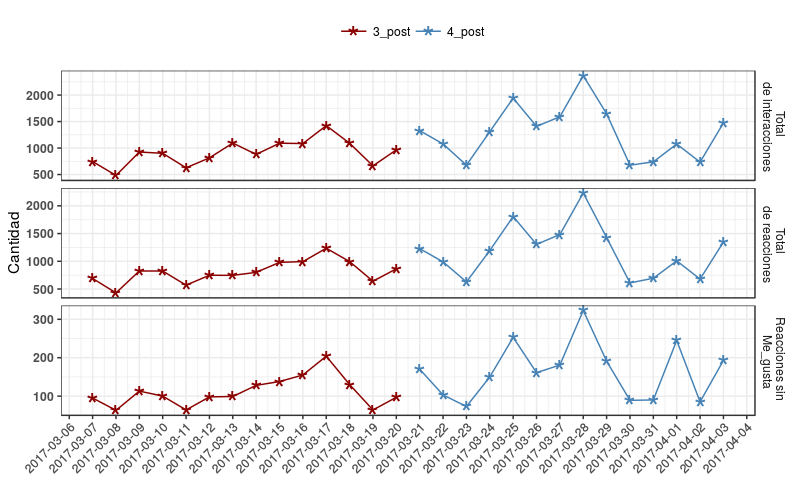
\includegraphics[width=.75\textwidth]{imagenes/graficas/historico1.png}
   \caption{Visión histórica de las interacciones principales.}
  \end{center} 
\end{figure}


\begin{figure}[H]
  \begin{center}
   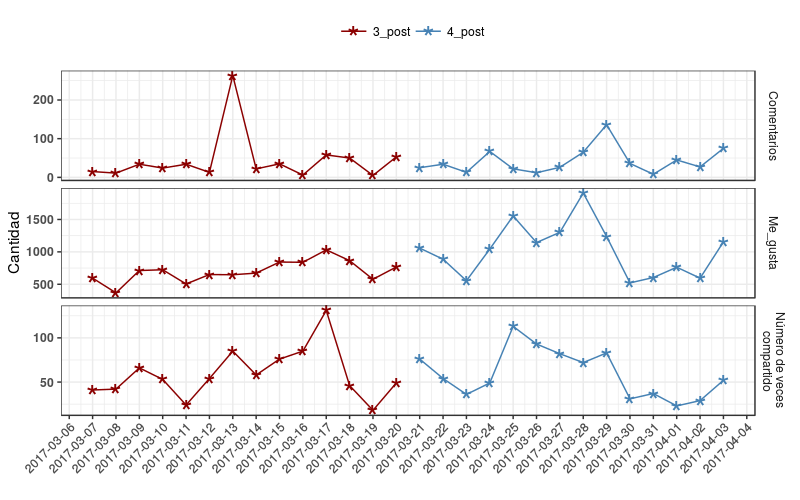
\includegraphics[width=.75\textwidth]{imagenes/graficas/historico2.png}
   \caption{Visión histórica de comentarios, ``Me gusta'' y Número de veces compartido.}
  \end{center}
\end{figure}

\begin{figure}[H]
  \begin{center}
   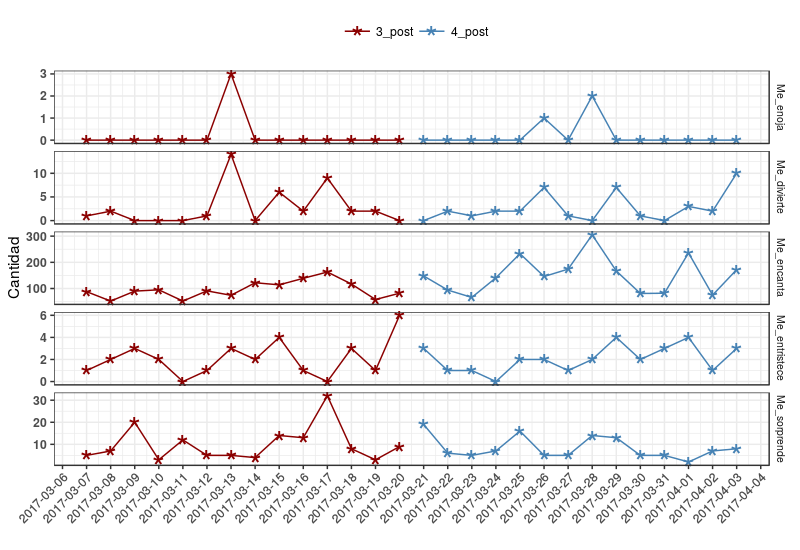
\includegraphics[width=.75\textwidth]{imagenes/graficas/historico3.png}
   \caption{Visión histórica de las reacciones de los posteos.}
  \end{center}
\end{figure}


\begin{figure}[H]
  \begin{center}
   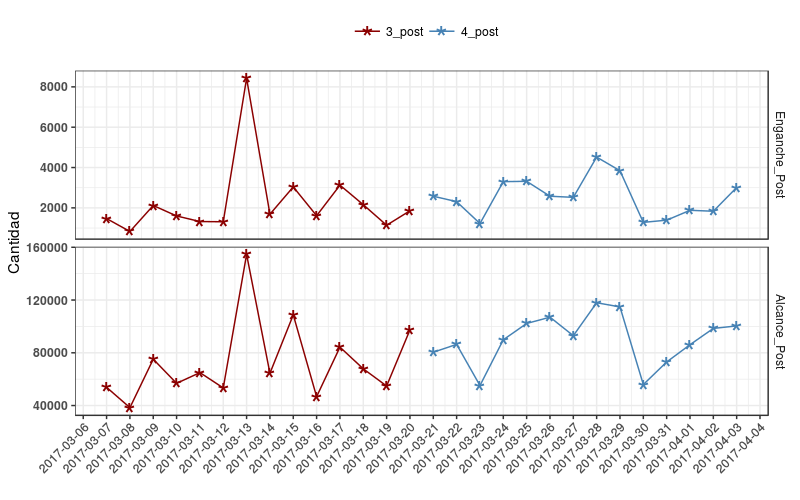
\includegraphics[width=.75\textwidth]{imagenes/graficas/historico4.png}
   \caption{Visión histórica del alcance y el enganche de los posteos.}
  \end{center}
\end{figure}

\begin{figure}[H]
  \begin{center}
   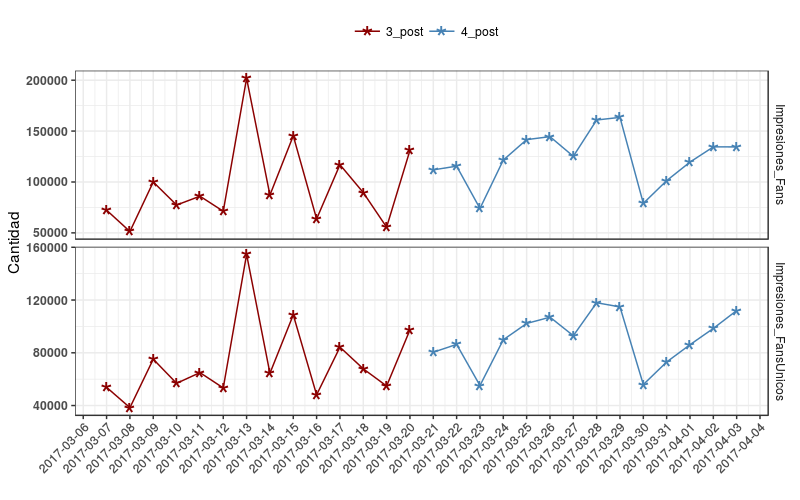
\includegraphics[width=.75\textwidth]{imagenes/graficas/historico5.png}
   \caption{Visión histórica de las impresiones del posteo hacia los fans (totales y únicas). }
  \end{center}
\end{figure}

\begin{figure}[H]
  \begin{center}
   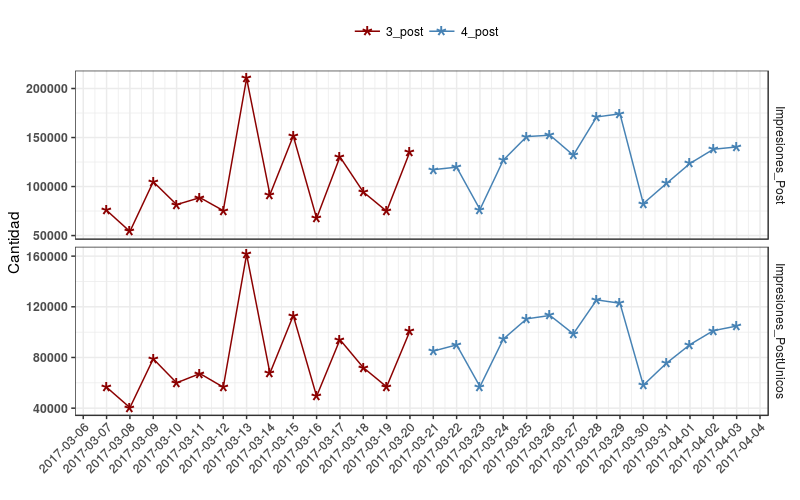
\includegraphics[width=.75\textwidth]{imagenes/graficas/historico6.png}
   \caption{Visión histórica de las impresiones del posteo (totales y únicas).}
  \end{center}
\end{figure}

\subsection{Comparación}
\subsubsection{Visión general de la comparación}
Se muestra el promedio, el máximo, el mínimo y el error estándar de las 
variables analizadas en este experimento.
\begin{center}
 \caption{Tabla1: Visión general.}
 {\footnotesize
  \begin{tabular} {c|c|c|c|c|c}
   \hline
   Tipo & Número de posteos & Promedio & Máximo & Mínimo & Error estándar \\
   \hline
   Interacción total  & 3  & 312 & 727  & 62 & 24.99 \\
   Interacción total  & 4  & 322 & 1310 & 7  & 32.94 \\
   Reacciones totales & 3  & 276 & 670  & 59 & 23.05 \\
   Reacciones totales & 4  & 296 & 1263 & 6  & 31.3 \\
   Reacciones sin ``Me gusta'' & 3  & 37 & 107 & 0 & 4.24 \\
   Reacciones sin ``Me gusta'' & 4  & 41 & 184 & 0 & 5.54 \\
   Número de comentarios & 3  & 15 & 239 & 0 & 5.77 \\
   Número de comentarios & 4  & 10 & 99  & 0 & 2.24 \\
   Número de veces compartido & 3  & 20 & 59 & 3 & 2.18 \\
   Número de veces compartido & 4  & 14 & 69 & 0 & 1.55 \\
   ``Me gusta'' & 3  & 238 & 572 & 58 & 19.13 \\
   ``Me gusta'' & 4  & 255 & 1084 & 6 & 26.2 \\
   ``Me encanta'' & 3  & 32 & 91 & 0 & 3.78 \\
   ``Me encanta'' & 4  & 37 & 178 & 0 & 5.25 \\
   ``Me divierte'' & 3  & 0.95 & 10 & 0 & 0.35 \\
   ``Me divierte'' & 4  & 0.67 & 7 & 0 & 0.2 \\
   ``Me sorprende'' & 3  & 3.41 & 22 & 0 & 0.73 \\
   ``Me sorprende'' & 4  & 2 & 10 & 0 & 0.32 \\
   ``Me enoja'' & 3  & 0.073 & 1 & 0 & 0.041 \\
   ``Me enoja'' & 4  & 0.053 & 2 & 0 & 0.039 \\
   ``Me entristece'' & 3  & 0.7 & 3 & 0 & 0.14 \\
   ``Me entristece'' & 4  & 0.51 & 2 & 0 & 0.09 \\
   Alcance posteo  & 3  & 24910 & 99525 & 7564 & 2386.17 \\
   Alcance posteo & 4 & 22512 & 54549 & 327 & 1218.72 \\
   Enganche posteo & 3  & 773 & 6636 & 113 & 156.28 \\
   Enganche posteo & 4  & 635 & 2535 & 25 & 62.91 \\
   Impresiones hacia los fans & 3  & 32916 & 124367 & 11222 & 2383.95 \\
   Impresiones hacia los fans & 4  & 30847 & 74493 & 477 &  1210.18 \\   
   Impresiones hacia los fans (únicos) & 3  & 24943 & 99525 & 7807 & 2383.95 \\
   Impresiones hacia los fans (únicos) & 4  & 22720 & 54549 & 327 & 1210.87 \\
   Impresiones de los posteos & 3  & 35045 & 128344 & 11552 & 3159.91 \\
   Impresiones de los posteos & 4  & 32301 & 79923  & 521 &  1804.74 \\
   Impresiones de los posteos (únicos) &  3  & 26219 & 103178 & 8009 & 2492.51 \\
   Impresiones de los posteos (únicos) & 4  & 23698 & 58672 & 366 & 1335.34 \\
   \hline    
  \end{tabular}
 }
\end{center}


\subsubsection{Interacción}
De manera general las interacciones totales, las reacciones totales y
las reacciones sin contar ``Me gusta'' muestran diferencias significativas 
(Tabla2 y Figura 8)

\begin{center}
 \caption{Tabla 2: Resumen del GLM de interacciones totales, reacciones totales y reacciones sin ``Me gusta''.} \\ [0.3cm]
 {\footnotesize
 \begin{tabular}{c|c|c|c|c}
  \hline 
  Tipo & Estimado & Error estándar & Valor de Z & \textit{P} \\
  \hline 
  \multicolumn{5}{c}{Interacciones totales} \\
  \hline
  Ordenada & 5.7 & 0.008 & 649.54 & 2e-16\\
  Comparación & 0.03 & 0.13 & 0.23 & 0.00472\\
  \hline 
  \multicolumn{5}{c}{Reacciones Totales} \\
  \hline
  Ordenada & 5.62 & 0.009 & 598.7 & 2e-16\\
  Comparacion & 0.07 & 0.012 & 5.83 & 5.36e-09\\
  \hline
  \multicolumn{5}{c}{Reacciones sin ``Me gusta''} \\
  \hline
  Ordenada & 3.63 & 0.02 & 142.86 & 2e-16\\
  Comparación & 0.08 & 0.003 & 2.65 & 0.00795 \\
  \hline

 \end{tabular}
 }	    
\end{center}

\begin{figure}[H]
 \begin{center}
    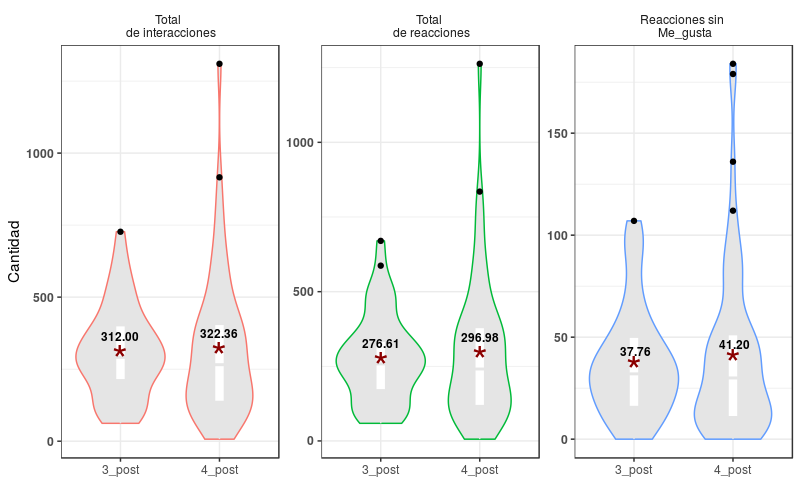
\includegraphics[width=.75\textwidth]{imagenes/graficas/comparacion1.png}
     \caption{Gráfico de violín que representa la comparación  entre semanas de las interacciones totales, reacciones totales, 
     y reacciones sin ``Me gusta'', se puede observar el promedio en forma de \textbf{*} y escrito en negritas.}
 \end{center}

\end{figure}


También resultaron significativos el número de veces compartido,  
``Me gusta'' y comentarios (Tabla 3 y Figura 9).

\begin{center}
 \caption{Tabla 3: Resumen del GLM de la comparación del  número de veces compartido, ``Me gusta'' y comentarios.} \\ [0.3cm]
 {\footnotesize
 \begin{tabular}{c|c|c|c|c}
  \hline 
  Tipo & Estimado & Error estándar & Valor de Z & \textit{P}\\
  \hline 
  \multicolumn{5}{c}{Número de veces compartido}\\
  \hline
  Ordenada & 3 & 0.03 & 86.48 & 2e-16 \\
  Comparación & -0.3 & 0.04 & -6.29 & 3.01e-10\\
  \hline 
  \multicolumn{5}{c}{``Me gusta''}\\
  \hline
  Ordenada & 5.47 &  0.01 & 541.88 & 2e-16 \\
  Comparación & 0.06 & 0.013 & 5.22 & 1.76e-07\\
  \hline
  \multicolumn{5}{c}{Número de comentarios}\\
  \hline
  Ordenada & 2.72 & 0.04 & 67.91 & 2e-16\\
  Comparación & -0.3 & 0.05 & -6.34 & 2.18e-10 \\
  \hline
 \end{tabular}
 }	    
\end{center}

\begin{figure}[H]
 \begin{center}
  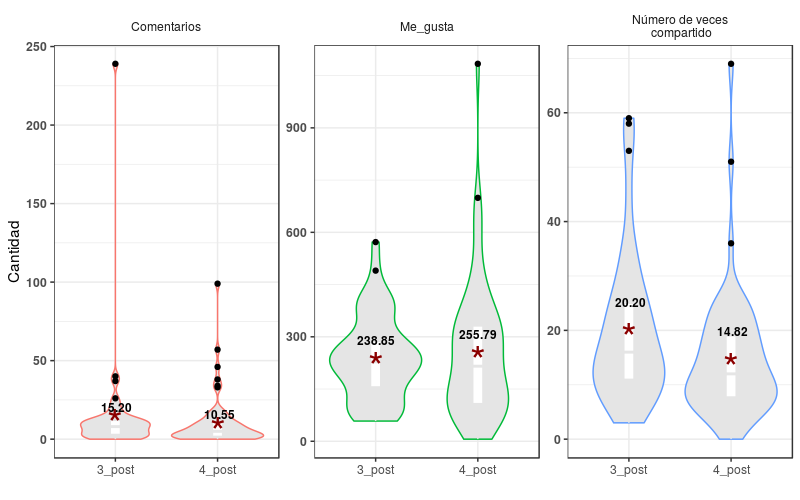
\includegraphics[width=.75\textwidth]{imagenes/graficas/comparacion2.png}
  \caption{Gráfico de violín representando la comparación entre semanas del número de veces compartido, ``Me gusta'' y comentarios,
  el \textbf{*} representa el promedio el cual está escrito en negritas.}
 \end{center}
\end{figure}


Con excepción de ``Me encanta'' y ``Me sorprende'' las demás reacciones resultaron
no significativas (Tabla 4 y Figura 10).

\begin{center}
 \caption{Tabla 4: Resumen del GLM de la comparación entre semanas de las reacciones de los posteos.} \\ [0.3cm]
 {\footnotesize
 \begin{tabular}{c|c|c|c|c}
  \hline 
  Tipo & Estimado & Error estándar & Valor de Z & \textit{P} \\
  \hline 
  \multicolumn{5}{c}{``Me encanta''} \\
  \hline
  Ordenada & 3.48 & 0.02 & 127.41 & 2e-16 \\
  Comparación & 0.14 & 0.03 & 4.272 & 1.93e-05 \\
  \hline 
  \multicolumn{5}{c}{``Me divierte''}\\
  \hline
  Ordenada & -0.05 & 0.16 & -0.31 & 0.755 \\
  Comparación & -0.33 & 0.22 & -1.48 & 0.138 \\
  \hline
  \multicolumn{5}{c}{``Me sorprende''}\\
  \hline
  Ordenada & 1.22 & 0.08 & 14.53 & 2e-16\\
  Comparación & -0..49 & 0.12 & -3.92 & 8.78e-05 \\
  \hline
  \multicolumn{5}{c}{``Me enoja''}\\
  \hline
  Ordenada & -2.61 & 0.57 & -4.52 & 5.92e-06\\
  Comparación & -0.31 & 0.81 & -0.38 & 0.7 \\
  \hline
  \multicolumn{5}{c}{``Me entristece''} \\
  \hline
  Ordenada & -0.34 & 0.18 & -1.86 & 0.062\\
  Comparación & -0.31 & 0.26 & 1.18 & 0.23 \\
  \hline
 \end{tabular}
 }	    
\end{center}

\begin{figure}[H]
 \begin{center}
  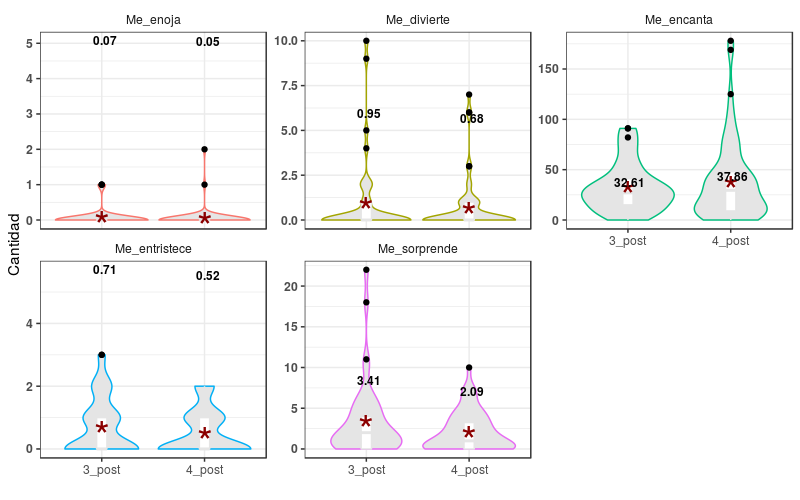
\includegraphics[width=.75\textwidth]{imagenes/graficas/comparacion3.png}
  \caption{Gráfico de violín que representa la comparación entre semanas de  las reacciones, 
  el \textbf{*} representa el promedio y está escrito en negritas.}
 \end{center}
\end{figure}


\subsubsection{Alcance, enganche e impresiones}
Para el caso del alcance y el enganche (Tabla 5 y Figura 11) y las 
impresiones únicas (Tabla 6 y Figura 12) y por posteo (Tabla 7 y Figura 13) ninguno
resultó significativo.

\begin{center}
 \caption{Tabla 5: Resumen del GLM de la comparación entre semanas del alcance y enganche por posteo.} \\ [0.3cm]
 {\footnotesize
 \begin{tabular}{c|c|c|c|c}
  \hline 
   Tipo &Estimado & Error estándar & Valor de T & \textit{P} \\
  \hline 
  \multicolumn{5}{c}{Alcance} \\
  \hline
  Ordenada & 10.12 & 0.07 & 131.14 & 2e-16 \\
  Comparación & -0.1 & 0.1 & -0.975 & 0.332 \\
  \hline 
  \multicolumn{5}{c}{Enganche}\\
  \hline
  Ordenada & 6.65 & 0.15 & 43.31 & 2e-16 \\
  Comparación & -0.91 & 0.21 & -0.928 & 0.356 \\
  \hline
  \end{tabular}
 }	    
\end{center}

\begin{figure}[H]
 \begin{center}
  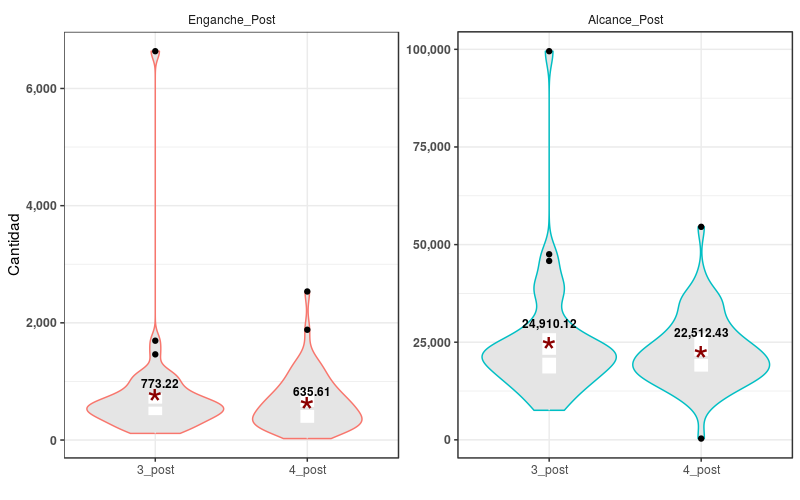
\includegraphics[width=.75\textwidth]{imagenes/graficas/comparacion4.png}
  \caption{Gráfico de violín representando la comparación entre semanas del  enganche y alcance por posteo,
  el \textbf{*} representa el promedio y está escrito en negritas.}
 \end{center}
\end{figure}


\begin{center}
 \caption{Tabla 6: Resumen del GLM de la comparación entre semanas de las impresiones hacia los fans, únicas y de manera general.} \\ [0.3cm]
 {\footnotesize
  \begin{tabular}{c|c|c|c|c}
   \hline
   Tipo & Estimado & Error estándar & Valor de T & \textit{P} \\
   \hline
   \multicolumn{5}{c}{Impresiones hacia los fans} \\
   \hline
   Ordenada & 10.4 & 0.07 & 136.4 & 2e-16 \\ 
   Comparacion & -0.06491 & 0.1 & -0.63 & 0.52 \\
   \hline
   \multicolumn{5}{c}{Impresiones hacia los fans (Únicos)} \\
   \hline
   Ordenada & 10.12 & 0.076 & 131.92 & 2e-16 \\
   Comparación & -0.09 & 0.1 & -0.9 & 0.36 \\
   \hline
  \end{tabular}
 }
\end{center}

\begin{figure}[H]
\begin{center}
 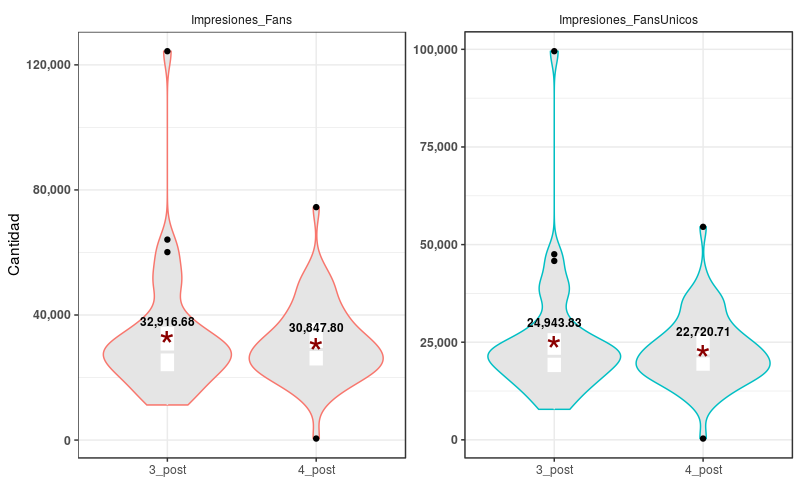
\includegraphics[width = .75\textwidth]{imagenes/graficas/comparacion5.png}
 \caption{Gráfico de violín de las comparaciones entre semanas de las impresiones hacia los fans,
 el \textbf{*} representa el promedio y está escrito en negritas.}
\end{center}
\end{figure}



\begin{center}
 \caption{Tabla 7: Resumen del GLM de la comparación entre semanas de las  impresiones de los posteos, únicas y de manera general.} \\[0.3cm]
 {\footnotesize
 \begin{tabular}{c|c|c|c|c}
  \hline
  Tipo & Estimado & Error estándar & Valor de T & \textit{P} \\
  \hline
  \multicolumn{5}{c}{Impresiones de los posteos} \\
  \hline
  Ordenada & 10.46 & 0.075 & 138.62 & 2e-16 \\
  Comparación & -0.08 & 0.1 & -0.8 & 0.42 \\
  \hline
  \multicolumn{5}{c}{Impresiones de los posteos (Únicos)} \\
  \hline
  Ordenada & 10.17 & 0.077 & 130.45 & 2e-16 \\
  Comparación & -0.1 & 0.1 & -0.96 & 0.33 \\
  \hline  
 \end{tabular}
 }
\end{center}

\begin{figure}[H]
 \begin{center}
  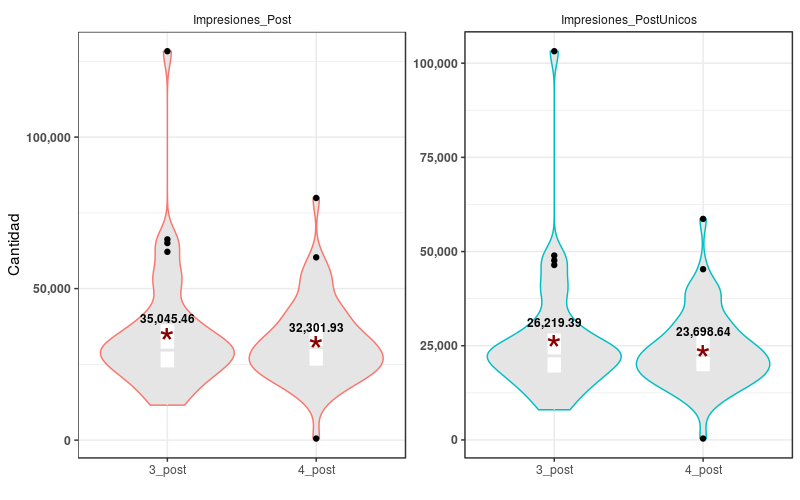
\includegraphics[width = .75\textwidth]{imagenes/graficas/comparacion6.png}
  \caption{Gráfico de violín de las comparaciones entre semanas de las impresiones de los posteos, el 
  \textbf{*} es el promedio y está escrito en negritas}
 \end{center}
\end{figure}

\subsection{Enganche general}
Para el caso del enganche en general, no se observaron diferencias significativas
entre semanas (Tabla 8 y Figura 14).

\begin{center}
 \caption{Tabla 8: Tabla de ANOVA  de las comparaciones del enganche por día}
 {\footnotesize
 \begin{tabular}{c|c|c|c|c|c}
 \hline
 Tipo & gl & Suma de cuadrados & Media cuadrática & Valor de F & \textit{P} \\
 \hline
 Comparación & 1 & 0.004 & 0.004 & 3.16 & 0.087 \\
 Residuales & 26 & 0.034 & 0.001 & & \\
 \hline
 \end{tabular}
 }
\end{center}

\begin{figure}[H]
 \begin{center}
  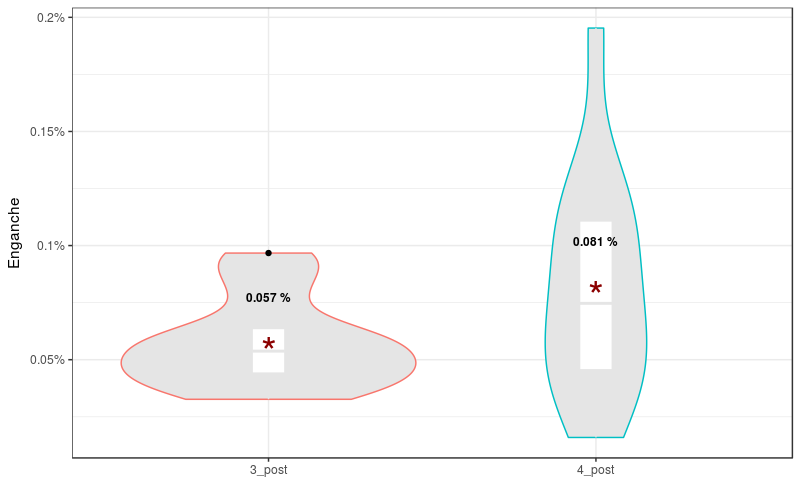
\includegraphics[width = .75\textwidth]{imagenes/graficas/comparacion7.png}
  \caption{Gráfico de violín que representa la comparación del porcentaje de enganche por día,
  el \textbf{*} representa el promedio y está escrito en negritas.}
 \end{center}
\end{figure}




\section{Discusión}
Los resultados muestran que métricas como el alcance, las impresiones y el enganche no
se ven afectados por la disminución de 1 posteo en la cuenta de Facebook de SEAT México. Esto parece coincidir
con lo dicho por Patel (2016) quien menciona que páginas con más de 10 mil seguidores tendrán un buen número
de ``Clicks'' y usuarios enganchados con tan solo dos posteos.
No obstante el número de interacciones (exceptuando:``Me enoja'', ``Me entristece'' y ``Me asombra'')
si se ve afectado, dando como resultado que cuatro posteos te generarán un mayor número de interacciones que tres.
Por lo que la estrategia de disminuir o mantener un determinado número  de posteos debe obedecer a las necesidades de la marca.
Esto debido a que si SEAT necesita mantener un  número similar  de usuarios enganchados y alcanzados,
puede disminuir el número de posteos, no obstante si su necesidad es obtener la mayor cantidad de interacciones posibles 
entonces es conveniente mantener el mismo número de posteos y en casos especiales, aumentar la cantidad de posteos por día.
Sin embargo, la cantidad de interacciones y usuarios enganchados puede ir de la mano con la calidad de las publicaciones, algo que 
no fue medido en el presente estudio.
De Vries (2012) propone una red conceptual  de variables que afectan el número de ``Me gusta'' y comentarios de los posteos,
dichas variables pueden ser controladas o no, para el caso de las variables controlables, se encuentran el día de la semana, 
la longitud del mensaje del posteo y la categoría del producto. Otras variables que menciona que pueden afectar
a la interacción de un posteo es la ``energía'' del mismo, la interactividad, la información adicional, el número
de comentarios positivos que genera y la posición del posteo al ser mostrado a un fan.

Todas estas variables deben ser tomadas en cuenta al momento de disminuir o mantener el número de posteos
de la página de SEAT, con el objetivo de mantener alcance, interacciones e impresiones y también aumentar o mantener
el número de interacciones de sus posteos.



\section{Conclusiones}
El disminuir o mantener el número de posteos por parte de SEAT debe de ir de la mano con sus objetivos.
Para este experimento el disminuir un posteo no afectó de manera significativa el número de personas alcanzadas o enganchadas por posteo.
Si se afectó el número de interacciones en general, dado que cuatro posteos generaron mayor interacción que tres.
Para futuros casos si se desea disminuir la cantidad de posteos, se deben de tomar en cuenta otras variables (calidad, interactividad)
para no afectar la interacción de la cuenta de SEAT. 


\begin{thebibliography}{10}
  \bibitem{1} Barbera P; Piccirilli M; Geisler A; Van Atteveldt W. (2017) Rfacebook: Access to Facebook API via R. R package version 0.6.13. https://github.com/pablobarbera/Rfacebook
  \bibitem{2} Casteleyn J; Mottart A; Rutten K. (2009). How to use Facebook in you market research. International Journal of Market Research. 51(4) 439-447.
  \bibitem{3} De Vries L; Gensler S; Leeflang P. (2012) Popularity of Brand Post on Brand Pages: An Investigation of the Effects of Social Media Marketing. Journal of interactive marketing. 26(2012) 83-91
  \bibitem{4} Facebook. (2016). \textit{ Statistics of  Facebook}, Palo  Alto,  CA:  Facebook. Tomado de: http://ltam.newsroom.fb.com/company-info/
  \bibitem{5} Facebook for developers (2017). Tomado de: https://developers.facebook.com/docs/graph-api
  \bibitem{6} Facebook business. (2013). Tomado de: https://www.facebook.com/business/news/News-Feed-FYI-A-Window-Into-News-Feed
  \bibitem{7} Internet World Stats. (2016). Tomado de: http://www.internetworldstats.com/stats.htm
  \bibitem{8} Nadkarni A; Hofmann S. (2012). Why Do People Use Facebook . Personality and Individual Differences. 52(2012) 243-249
  \bibitem{9} Patel N. (2012). How Frequently You Should Post on Social Media According to the Pros. Forbes. Tomado de: http://www.forbes.com/sites/neilpatel/2016/09/12/how-frequently-you-should-post-on-social-media-according-to-the-pros/#3d7172ca36d5
  \bibitem{10} R Core Team (2017). R: A language and environment for statistical computing. R Foundation for Statistical Computing, Vienna, Austria. URL https://www.R-project.org/
  \bibitem{11} Roshnee R; Fowdar S. (2013). The implications of Facebook Marketing for Organizations. Contemporay Management Research. 9 (1) 73-84. doi:10.7903/cmr.9710
  \bibitem{12} Smarth Insights. (2016). Global social media research summary 2016. Tomado de: http://www.smartinsights.com/social-media-marketing/social-media-strategy/new-global-social-media-research/
  \bibitem{13}  Wickham H. (2009). ggplot2: Elegant Graphics for Data Analysis. Springer-Verlag New York	
  \bibitem{14} Wilson R; Gosling S; Graham L. (2012). A review of Facebook research in the social sciences. Perspectives on Psychological Science 7 (3) 203-220
  \bibitem{15} Zar J. (2010). Biostatistical Analysis. Pearson Prentice Hall. New Jersey. ISBN-10: 0-13-100846-3
\end{thebibliography}

\end{document}
